\section*{Results}

%Результаты, как двигается, численные показатели силы
\begin{figure}[H]
    \centering
    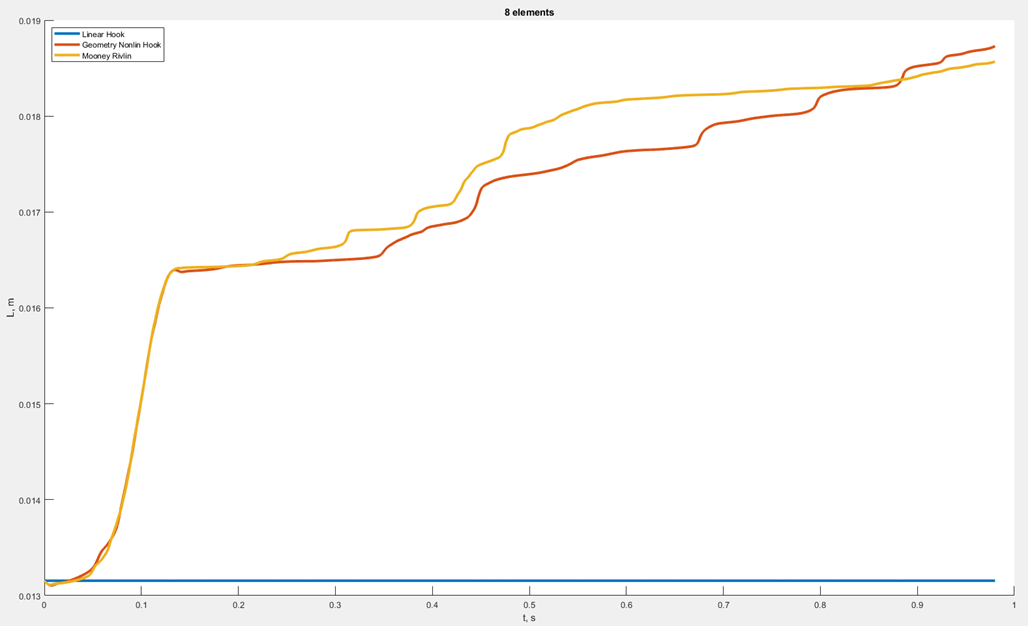
\includegraphics[width=\columnwidth]{./fig/comparePhMods.png}
    \caption{8 elements, Linear Hooke(blue), Nonlinear geometry Hooke(red),
     Mooney-Rivlin(yellow)}
    \label{fig:MT}
\end{figure}
\newpage
\begin{figure}[H]
    \centering
    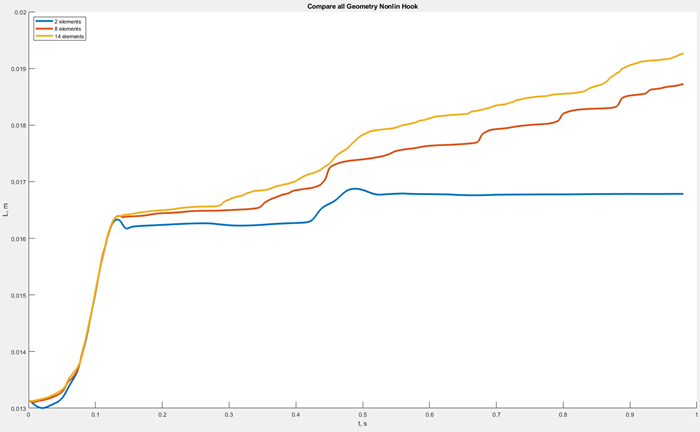
\includegraphics[width=\columnwidth]{./fig/geomNon.png}
    \caption{Nonlinear geometry Hooke model, 2(blue), 8(red), 14(yellow) elements}
    \label{fig:MT}
\end{figure}
\newpage

\begin{figure}[H]
    \centering
    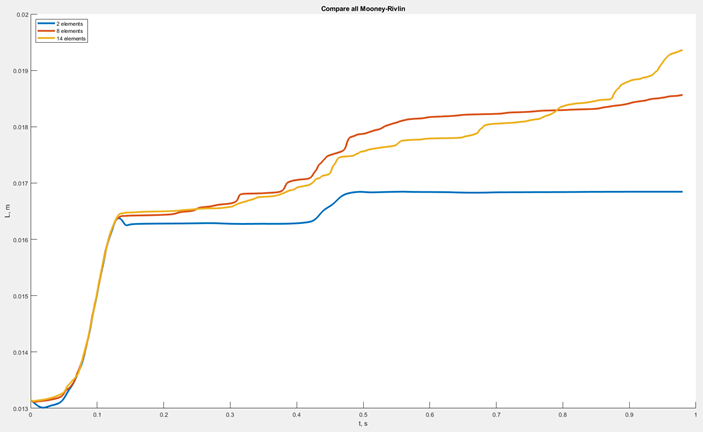
\includegraphics[width=\columnwidth]{./fig/mooneyRivlin.png}
    \caption{Nonlinear Mooney-Rivlin model, 2(blue), 8(red), 14(yellow) elements}
    \label{fig:MT}
\end{figure}
\newpage
